\documentclass[11pt]{beamer}
\usepackage{keynote-portfolio} 
	
% * * * * * * * * * * * * * * INCLUDE  * * * * * * * * * * * * * * * * *
\usepackage[T1]{fontenc} 
\usepackage[utf8]{inputenc}
\usepackage[frenchb]{babel}
\usepackage{amsmath}
\usepackage{xcolor}  
\usepackage{graphicx}
\usepackage{animate}
\usepackage{movie15}  
\usepackage{tikz}

% * * * * * * * * * * * * * LA BARRE DE NAVIGATION  * * * * * * * * * * * * * *
\setbeamertemplate{navigation symbols}{%
	\insertslidenavigationsymbol%
	\insertframenavigationsymbol%
	\insertdocnavigationsymbol%
	\insertbackfindforwardnavigationsymbol%
}

% * * * * * * * * * * * * * * * * * TEXTPOS * * * * * * * * * * * * * * * * * *
\usepackage[absolute,showboxes,overlay]{textpos}
\TPshowboxestrue                                              % affiche le contour des textblocks	
\TPshowboxesfalse                                             % fait disparaitre le contour des textblocks
\textblockorigin{2mm}{8mm}                                    % origine des positions pour placer les textblocks

% * * * * * * * * * * * * * * * * * PICTURE * * * * * * * * * * * * * * * * * *
\usepackage{picture}
\setlength{\unitlength}{1mm}  

% * * * * * * * * * * * * * DETAILS DE STYLE  * * * * * * * * * * * * * * * * *
%\beamertemplatetransparentcovered      
\setbeamertemplate{itemize item}[ball] 
\setbeamertemplate{itemize subitem}[triangle] 
\renewcommand{\footnoterule}{}
\renewcommand{\thefootnote}{\alph{footnote}}   

% * * * * * * * * * * * * * *  PAGES DE TITRE * * * * * * * * * * * * * * * * *
%\title[Google Summer of Code]{Google Summer of Code}
\author[Erwan Douaille]{Erwan Douaille}
\institute{University of Lille 1}
\date{9th october 2013}


% * * * * * * * * * * * * * PARAMETRES POUR PDF * * * * * * * * * * * * * * * *
\hypersetup{% Modifiez la valeur des champs suivants
	pdfauthor   = {Erwan Douaille},
	pdftitle    = {Google Summer of Code},
	pdfsubject  = {},
	pdfkeywords = {Google Summer of Code Erwan Douaille Pharo},
	pdfcreator  = {PDFLaTeX},
	pdfproducer = {PDFLaTeX},
	pdfpagemode = {FullScreen}
}

% * * * * * * * * * * * * * * * * * * * * * * * * * * * * * * * * * * * * * * *
% * * * * * * * * * * * * * *  DEBUT DOCUMENT * * * * * * * * * * * * * * * * *
% * * * * * * * * * * * * * * * * * * * * * * * * * * * * * * * * * * * * * * *

\begin{document}


% --------- Page de garde ---------
\begin{frame} 
	\hbox{ 
     	\hspace*{2cm}
		
\includegraphics[scale=0.20]{images/gsoc.jpg}
	}
	\titlepage
\end{frame}
% ----------------------------

% --------- Sommaire ---------
\begin{frame}{Contents}
	\tableofcontents[]
\end{frame}      
% ----------------------------


\section{Presentation}
\begin{frame}{Presentation}
	\begin{itemize}
		\item Annual program
		\item Promotes the open source community, such as Linux Debian Python ...
		\item Awards students
		\item Since 2004
		\item Summer of Love
		\item Skills ?
	\end{itemize}
\end{frame}


\section{Benefits}
\begin{frame}{Benefits}
	"Flip bits, not burgers"
		\hbox{ 
     		\hspace*{4cm}
		
\includegraphics[scale=0.26]{images/code.png}	
		}
	\begin{itemize}
		\item Inspire young developers to begin participating in open source development
		\item Money 5000 USD
		\item Beef Up Your Resume, 1192 students 2013
		\item Free time, ~2 month
		\item Skills
		\item Real World Experience
		\item Contacts
	\end{itemize}
\end{frame}
	

\section{Limitations}
\begin{frame}{Limitations}
	\begin{itemize}
		\item GSoC 2014, 19th may - 22th august
		\item Sleepless night
		\item Evaluations
	\end{itemize}
\end{frame}


\section{My project}
\begin{frame}{My project}
		\hbox{ 
     		\hspace*{5cm}
			
\includegraphics[scale=0.3]{images/esug.png}
		}
	\begin{itemize}
		\item Smalltalk 
		\item UIPainter, tool to create in an easy way GUI
	\end{itemize}
	\begin{center}
		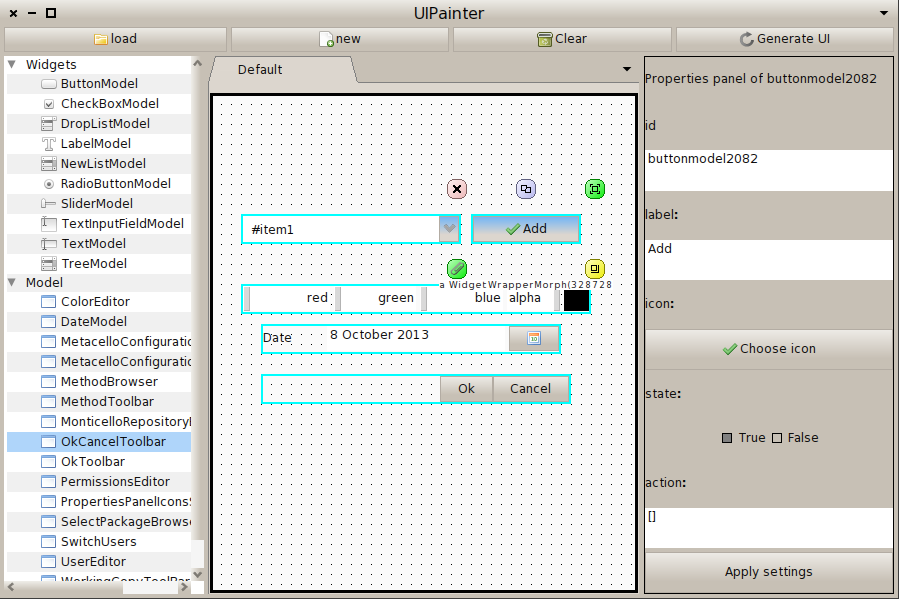
\includegraphics[scale=0.28]{images/uipainter.png}	
	\end{center}
\end{frame}

\begin{frame}{Conclusion}
	\begin{columns}[T]
    		\begin{column}{.45\textwidth}
    			\begin{block}{Memo}
    				\begin{itemize}
    					\item Have fun
    					\item Beef Up Your Resume
    					\item Awards and money
    					\item Contributor
    				\end{itemize}
    			\end{block}
    		\end{column}
    		\begin{column}{.5\textwidth}
   			\begin{block}{Want to try it ??}
   				\begin{itemize}
   					\item Start proposals in march 2014
   					\item \href{http://www.google-melange.com/}{www.google-melange.com}	
   					\item Maybe a presentation is coming at Lille 1
   				\end{itemize}   				
    			\end{block}
    		\end{column}
  \end{columns}
\end{frame}


\end{document}
